% Standalone TikZ figure: O(1) Temporal Scaling
% Shows computational cost vs time horizon for different evolution methods
\documentclass[tikz,border=5pt]{standalone}
\usepackage{amsmath,amssymb}
\usepackage{pgfplots}
\pgfplotsset{compat=1.18}

\definecolor{hdcblue}{HTML}{0072B2}
\definecolor{ltcorange}{HTML}{E69F00}
\definecolor{eulerred}{HTML}{D55E00}
\definecolor{rk4purple}{HTML}{CC79A7}
\definecolor{itergreen}{HTML}{009E73}

\begin{document}

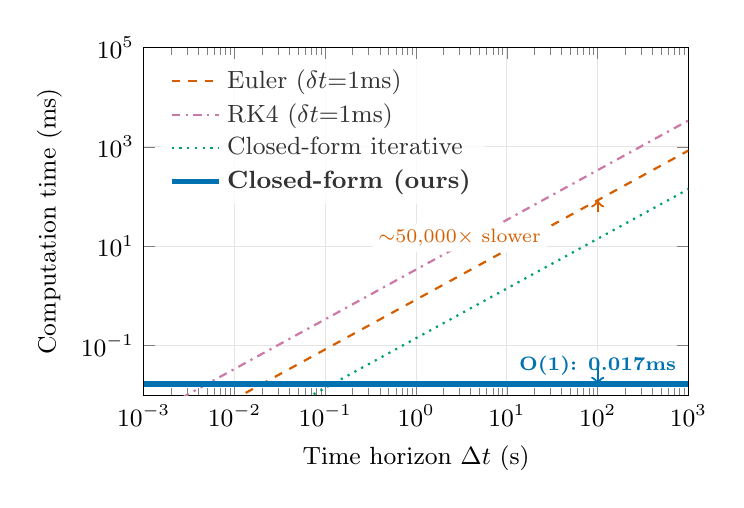
\begin{tikzpicture}
\begin{axis}[
    width=8.5cm,
    height=6cm,
    xlabel={Time horizon $\Delta t$ (s)},
    ylabel={Computation time (ms)},
    xmode=log,
    ymode=log,
    xmin=0.001, xmax=1000,
    ymin=0.01, ymax=100000,
    grid=major,
    grid style={gray!20},
    legend pos=north west,
    legend cell align=left,
    legend style={font=\small, draw=none, fill=white, fill opacity=0.8},
    tick label style={font=\small},
    label style={font=\small},
    every axis plot/.append style={thick},
]

% Euler: linear in dt, with step size delta=1ms
% Cost = D * (dt / delta) * c_euler, where c_euler gives 847ms for 1000 steps at D=16384
% 847ms for dt=1s (1000 steps), so cost_per_step = 0.847ms
% cost = 0.847 * dt/0.001
\addplot[eulerred, dashed, mark=none, domain=0.001:1000, samples=100]
    {0.847 * x};
\addlegendentry{Euler ($\delta t{=}1$ms)}

% RK4: linear in dt, 4x per step
% 3412ms for dt=1s, so cost = 3.412 * dt
\addplot[rk4purple, dashdotted, mark=none, domain=0.001:1000, samples=100]
    {3.412 * x};
\addlegendentry{RK4 ($\delta t{=}1$ms)}

% Closed-form iterative: linear but with larger step (tau/10)
% 0.142ms for 1s, cost = 0.142 * dt
\addplot[itergreen, dotted, mark=none, domain=0.001:1000, samples=100]
    {0.142 * x};
\addlegendentry{Closed-form iterative}

% Our closed-form: CONSTANT at 0.017ms regardless of dt
\addplot[hdcblue, solid, line width=2pt, mark=none, domain=0.001:1000, samples=100]
    {0.017};
\addlegendentry{\textbf{Closed-form (ours)}}

% Annotations
\node[font=\scriptsize, hdcblue, fill=white, inner sep=2pt, rounded corners=1pt]
    at (axis cs: 100, 0.04) {\textbf{O(1): 0.017ms}};
\node[font=\scriptsize, eulerred, fill=white, inner sep=2pt, rounded corners=1pt]
    at (axis cs: 3, 15) {$\sim$50{,}000$\times$ slower};

% Arrow showing gap at dt=100s
\draw[->, hdcblue, thick] (axis cs: 100, 0.05) -- (axis cs: 100, 0.017);
\draw[->, eulerred, thick] (axis cs: 100, 50) -- (axis cs: 100, 84.7);

\end{axis}
\end{tikzpicture}

\end{document}
